% This file was created by matlab2tikz.
%
%The latest updates can be retrieved from
%  http://www.mathworks.com/matlabcentral/fileexchange/22022-matlab2tikz-matlab2tikz
%where you can also make suggestions and rate matlab2tikz.
%
\definecolor{mycolor1}{rgb}{0.00000,0.44700,0.74100}%
%
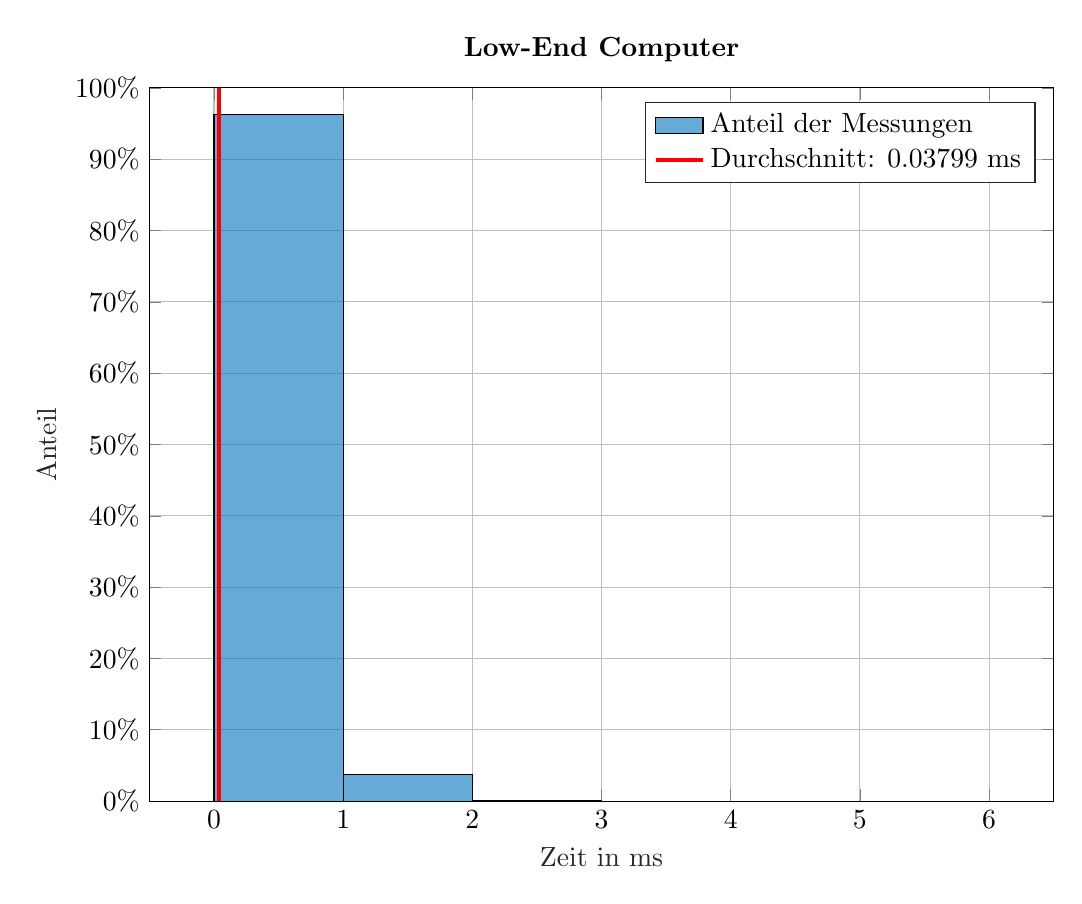
\begin{tikzpicture}

\begin{axis}[%
width=4.521in,
height=3.566in,
at={(0.758in,0.481in)},
scale only axis,
xmin=-0.5,
xmax=6.5,
xtick={0, 1, 2, 3, 4, 5, 6},
xlabel style={font=\color{white!15!black}},
xlabel={Zeit in ms},
ymin=0,
ymax=1,
ytick={0,0.1,0.2,0.3,0.4,0.5,0.6,0.7,0.8,0.9,1},
yticklabels={{0\%},{10\%},{20\%},{30\%},{40\%},{50\%},{60\%},{70\%},{80\%},{90\%},{100\%}},
ylabel style={font=\color{white!15!black}},
ylabel={Anteil},
axis background/.style={fill=white},
title style={font=\bfseries},
title={Low-End Computer},
xmajorgrids,
ymajorgrids,
legend style={legend cell align=left, align=left, draw=white!15!black}
]
\addplot[ybar interval, fill=mycolor1, fill opacity=0.6, draw=black, area legend] table[row sep=crcr] {%
x	y\\
0	0.962838461538462\\
1	0.0370230769230769\\
2	0.000107692307692308\\
3	7.69230769230769e-06\\
4	0\\
5	0\\
6	7.69230769230769e-06\\
7	0\\
8	0\\
9	0\\
10	0\\
11	7.69230769230769e-06\\
12	0\\
13	0\\
14	0\\
15	0\\
16	0\\
17	0\\
18	0\\
19	0\\
20	0\\
21	0\\
22	0\\
23	0\\
24	0\\
25	0\\
26	0\\
27	0\\
28	0\\
29	0\\
30	0\\
31	0\\
32	0\\
33	0\\
34	0\\
35	0\\
36	0\\
37	0\\
38	0\\
39	0\\
40	0\\
41	0\\
42	0\\
43	0\\
44	0\\
45	0\\
46	0\\
47	0\\
48	0\\
49	0\\
50	0\\
51	0\\
52	0\\
53	0\\
54	0\\
55	0\\
56	0\\
57	0\\
58	0\\
59	0\\
60	0\\
61	0\\
62	0\\
63	0\\
64	0\\
65	0\\
66	0\\
67	0\\
68	0\\
69	0\\
70	0\\
71	0\\
72	0\\
73	0\\
74	0\\
75	0\\
76	0\\
77	7.69230769230769e-06\\
78	7.69230769230769e-06\\
};
\addlegendentry{Anteil der Messungen}

\addplot [color=red, line width=1.5pt]
  table[row sep=crcr]{%
0.0379923076923077	0\\
0.0379923076923077	1\\
};
\addlegendentry{Durchschnitt: 0.03799 ms}

\end{axis}
\end{tikzpicture}%